%------------------------------------------------------------------------
%Editar Diplomado
\hypertarget{cv:GestionarPasos}{\section{Gestionar Pasos}} \label{sec:GestionarPasos}

	Esta funcionalidad le permitirá las acciones necesarias para controlar los pasos pertenecientes a una trayectoria y visualizarlos en una tabla en el proyecto sobre el que se está operando y solicitar el registro de uno nuevo.

		\subsection{Procedimiento}

			%Pasos de procedimiento
			\begin{enumerate}
			
			\item Oprima el botón \IUPasos{} de algún registro existente de la pantalla \ref{fig:GestionarTrayectorias} ''Gestionar Trayectorias''.
	
			\item Se mostrará la pantalla \ref{fig:GestionarPasos} ''Gestionar Pasos''.

			%Pantalla
			\begin{figure}[htbp!]
				\begin{center}
					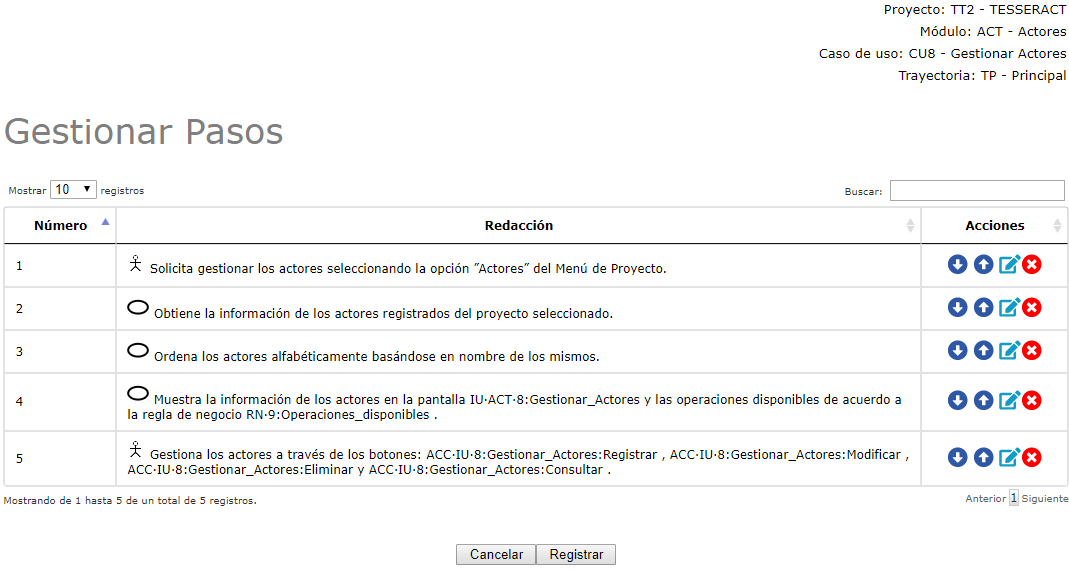
\includegraphics[scale=0.6]{roles/lider/casosUso/trayectorias/pasos/pantallas/iu6-1-1-1-1-1gestionarPasos}
					\caption{Gestionar Pasos}
					\label{fig:GestionarPasos}
				\end{center}
			\end{figure}
		
			\item Si es el caso puede cambiar de orden los pasos registrados mediante los botones PENDIENTE.
		
			\item Seleccione la operación que desea realizar:
			
			Para (\hyperlink{cv:registrarPaso}{Registrar}) dé clic en el botón \IURegistrar.
			
			Para (\hyperlink{cv:modificarPaso}{Modificar}) dé clic en el icono \IUEditar{} de algún paso ya registrado.
			
			Para (\hyperlink{cv:eliminarPaso}{Eliminar}) dé clic en el icono \IUBotonEliminar{} de algún paso ya registrado.
			
			\end{enumerate}